% !Mode:: "TeX:UTF-8"
\documentclass[12pt,a4paper]{article}

%%%%%%%%------------------------------------------------------------------------
%%%% 日常所用宏包

%% 控制页边距
% 如果是beamer文档类, 则不用geometry
\makeatletter
\@ifclassloaded{beamer}{}{\usepackage[top=2.5cm, bottom=2.5cm, left=2.5cm, right=2.5cm]{geometry}}
\makeatother

%% 控制项目列表
\usepackage{enumerate}

%% 多栏显示
\usepackage{multicol}

%% 算法环境
\usepackage{algorithm}  
\usepackage{algorithmic} 
\usepackage{float} 

%% 网址引用
\usepackage{url}

%% 控制矩阵行距
\renewcommand\arraystretch{1.4}

%% hyperref宏包,生成可定位点击的超链接,并且会生成pdf书签
\makeatletter
\@ifclassloaded{beamer}{
\usepackage{hyperref}
\usepackage{ragged2e} % 对齐
}{
\usepackage[%
    pdfstartview=FitH,%
    CJKbookmarks=true,%
    bookmarks=true,%
    bookmarksnumbered=true,%
    bookmarksopen=true,%
    colorlinks=true,%
    citecolor=blue,%
    linkcolor=blue,%
    anchorcolor=green,%
    urlcolor=blue%
]{hyperref}
}
\makeatother



\makeatletter % 如果是 beamer 不需要下面两个包
\@ifclassloaded{beamer}{
\mode<presentation>
{
} 
}{
%% 控制标题
\usepackage{titlesec}
%% 控制目录
\usepackage{titletoc}
}
\makeatother

%% 控制表格样式
\usepackage{booktabs}

%% 控制字体大小
\usepackage{type1cm}

%% 首行缩进,用\noindent取消某段缩进
\usepackage{indentfirst}

%%边框
\usepackage{listings}

%% 支持彩色文本、底色、文本框等
\usepackage{color,xcolor}

%% AMS LaTeX宏包: http://zzg34b.w3.c361.com/package/maths.htm#amssymb
\usepackage{amsmath,amssymb}
%% 多个图形并排
\usepackage{subfig}
%%%% 基本插图方法
%% 图形宏包
\usepackage{graphicx}
\newcommand{\red}[1]{\textcolor{red}{#1}}
\newcommand{\blue}[1]{\structure{#1}}
\newcommand{\brown}[1]{\textcolor{brown}{#1}}
\newcommand{\green}[1]{\textcolor{green}{#1}}


%%%% 基本插图方法结束

%%%% pgf/tikz绘图宏包设置
\usepackage{pgf,tikz}
\usetikzlibrary{shapes,automata,snakes,backgrounds,arrows}
\usetikzlibrary{mindmap}
%% 可以直接在latex文档中使用graphviz/dot语言,
%% 也可以用dot2tex工具将dot文件转换成tex文件再include进来
%% \usepackage[shell,pgf,outputdir={docgraphs/}]{dot2texi}
%%%% pgf/tikz设置结束


\makeatletter % 如果是 beamer 不需要下面两个包
\@ifclassloaded{beamer}{

}{
%%%% fancyhdr设置页眉页脚
%% 页眉页脚宏包
\usepackage{fancyhdr}
%% 页眉页脚风格
\pagestyle{plain}
}

%% 有时会出现\headheight too small的warning
\setlength{\headheight}{15pt}

%% 清空当前页眉页脚的默认设置
%\fancyhf{}
%%%% fancyhdr设置结束


\makeatletter % 对 beamer 要重新设置
\@ifclassloaded{beamer}{

}{
%%%% 设置listings宏包用来粘贴源代码
%% 方便粘贴源代码,部分代码高亮功能
\usepackage{listings}

%% 设置listings宏包的一些全局样式
%% 参考http://hi.baidu.com/shawpinlee/blog/item/9ec431cbae28e41cbe09e6e4.html
\lstset{
showstringspaces=false,              %% 设定是否显示代码之间的空格符号
numbers=left,                        %% 在左边显示行号
numberstyle=\tiny,                   %% 设定行号字体的大小
basicstyle=\footnotesize,                    %% 设定字体大小\tiny, \small, \Large等等
keywordstyle=\color{blue!70}, commentstyle=\color{red!50!green!50!blue!50},
                                     %% 关键字高亮
frame=shadowbox,                     %% 给代码加框
rulesepcolor=\color{red!20!green!20!blue!20},
escapechar=`,                        %% 中文逃逸字符,用于中英混排
xleftmargin=2em,xrightmargin=2em, aboveskip=1em,
breaklines,                          %% 这条命令可以让LaTeX自动将长的代码行换行排版
extendedchars=false                  %% 这一条命令可以解决代码跨页时,章节标题,页眉等汉字不显示的问题
}}
\makeatother
%%%% listings宏包设置结束


%%%% 附录设置
\makeatletter % 对 beamer 要重新设置
\@ifclassloaded{beamer}{

}{
\usepackage[title,titletoc,header]{appendix}
}
\makeatother
%%%% 附录设置结束


%%%% 日常宏包设置结束
%%%%%%%%------------------------------------------------------------------------


%%%%%%%%------------------------------------------------------------------------
%%%% 英文字体设置结束
%% 这里可以加入自己的英文字体设置
%%%%%%%%------------------------------------------------------------------------

%%%%%%%%------------------------------------------------------------------------
%%%% 设置常用字体字号,与MS Word相对应

%% 一号, 1.4倍行距
\newcommand{\yihao}{\fontsize{26pt}{36pt}\selectfont}
%% 二号, 1.25倍行距
\newcommand{\erhao}{\fontsize{22pt}{28pt}\selectfont}
%% 小二, 单倍行距
\newcommand{\xiaoer}{\fontsize{18pt}{18pt}\selectfont}
%% 三号, 1.5倍行距
\newcommand{\sanhao}{\fontsize{16pt}{24pt}\selectfont}
%% 小三, 1.5倍行距
\newcommand{\xiaosan}{\fontsize{15pt}{22pt}\selectfont}
%% 四号, 1.5倍行距
\newcommand{\sihao}{\fontsize{14pt}{21pt}\selectfont}
%% 半四, 1.5倍行距
\newcommand{\bansi}{\fontsize{13pt}{19.5pt}\selectfont}
%% 小四, 1.5倍行距
\newcommand{\xiaosi}{\fontsize{12pt}{18pt}\selectfont}
%% 大五, 单倍行距
\newcommand{\dawu}{\fontsize{11pt}{11pt}\selectfont}
%% 五号, 单倍行距
\newcommand{\wuhao}{\fontsize{10.5pt}{10.5pt}\selectfont}
%%%%%%%%------------------------------------------------------------------------


%% 设定段间距
\setlength{\parskip}{0.5\baselineskip}

%% 设定行距
\linespread{1}


%% 设定正文字体大小
% \renewcommand{\normalsize}{\sihao}

%制作水印
\RequirePackage{draftcopy}
\draftcopyName{XTUMESH}{100}
\draftcopySetGrey{0.90}
\draftcopyPageTransform{40 rotate}
\draftcopyPageX{350}
\draftcopyPageY{80}

%%%% 个性设置结束
%%%%%%%%------------------------------------------------------------------------


%%%%%%%%------------------------------------------------------------------------
%%%% bibtex设置

%% 设定参考文献显示风格
% 下面是几种常见的样式
% * plain: 按字母的顺序排列,比较次序为作者、年度和标题
% * unsrt: 样式同plain,只是按照引用的先后排序
% * alpha: 用作者名首字母+年份后两位作标号,以字母顺序排序
% * abbrv: 类似plain,将月份全拼改为缩写,更显紧凑
% * apalike: 美国心理学学会期刊样式, 引用样式 [Tailper and Zang, 2006]

\makeatletter
\@ifclassloaded{beamer}{
\bibliographystyle{apalike}
}{
\bibliographystyle{unsrt}
}
\makeatother


%%%% bibtex设置结束
%%%%%%%%------------------------------------------------------------------------

%%%%%%%%------------------------------------------------------------------------
%%%% xeCJK相关宏包

\usepackage{xltxtra,fontspec,xunicode}
\usepackage[slantfont, boldfont]{xeCJK} 

\setlength{\parindent}{2em}%中文缩进两个汉字位

%% 针对中文进行断行
\XeTeXlinebreaklocale "zh"             

%% 给予TeX断行一定自由度
\XeTeXlinebreakskip = 0pt plus 1pt minus 0.1pt

%%%% xeCJK设置结束                                       
%%%%%%%%------------------------------------------------------------------------

%%%%%%%%------------------------------------------------------------------------
%%%% xeCJK字体设置

%% 设置中文标点样式,支持quanjiao、banjiao、kaiming等多种方式
\punctstyle{kaiming}                                        
                                                     
%% 设置缺省中文字体
%\setCJKmainfont[BoldFont={Adobe Heiti Std}, ItalicFont={Adobe Kaiti Std}]{Adobe Song Std}   
\setCJKmainfont{SimSun}
%% 设置中文无衬线字体
%\setCJKsansfont[BoldFont={Adobe Heiti Std}]{Adobe Kaiti Std}  
%% 设置等宽字体
%\setCJKmonofont{Adobe Heiti Std}                            

%% 英文衬线字体
\setmainfont{DejaVu Serif}                                  
%% 英文等宽字体
\setmonofont{DejaVu Sans Mono}                              
%% 英文无衬线字体
\setsansfont{DejaVu Sans}                                   

%% 定义新字体
\setCJKfamilyfont{song}{Adobe Song Std}                     
\setCJKfamilyfont{kai}{Adobe Kaiti Std}
\setCJKfamilyfont{hei}{Adobe Heiti Std}
\setCJKfamilyfont{fangsong}{Adobe Fangsong Std}
\setCJKfamilyfont{lisu}{LiSu}
\setCJKfamilyfont{youyuan}{YouYuan}

%% 自定义宋体
\newcommand{\song}{\CJKfamily{song}}                       
%% 自定义楷体
\newcommand{\kai}{\CJKfamily{kai}}                         
%% 自定义黑体
\newcommand{\hei}{\CJKfamily{hei}}                         
%% 自定义仿宋体
\newcommand{\fangsong}{\CJKfamily{fangsong}}               
%% 自定义隶书
\newcommand{\lisu}{\CJKfamily{lisu}}                       
%% 自定义幼圆
\newcommand{\youyuan}{\CJKfamily{youyuan}}                 

%%%% xeCJK字体设置结束
%%%%%%%%------------------------------------------------------------------------

%%%%%%%%------------------------------------------------------------------------
%%%% 一些关于中文文档的重定义
\newcommand{\chntoday}{\number\year\,年\,\number\month\,月\,\number\day\,日}
%% 数学公式定理的重定义

%% 中文破折号,据说来自清华模板
\newcommand{\pozhehao}{\kern0.3ex\rule[0.8ex]{2em}{0.1ex}\kern0.3ex}

\newtheorem{example}{例}                                   
\newtheorem{theorem}{定理}[section]                         
\newtheorem{definition}{定义}
\newtheorem{axiom}{公理}
\newtheorem{property}{性质}
\newtheorem{proposition}{命题}
\newtheorem{lemma}{引理}
\newtheorem{corollary}{推论}
\newtheorem{remark}{注解}
\newtheorem{condition}{条件}
\newtheorem{conclusion}{结论}
\newtheorem{assumption}{假设}

\makeatletter %
\@ifclassloaded{beamer}{

}{
%% 章节等名称重定义
\renewcommand{\contentsname}{目录}     
\renewcommand{\indexname}{索引}
\renewcommand{\listfigurename}{插图目录}
\renewcommand{\listtablename}{表格目录}
\renewcommand{\appendixname}{附录}
\renewcommand{\appendixpagename}{附录}
\renewcommand{\appendixtocname}{附录}
%% 设置chapter、section与subsection的格式
\titleformat{\chapter}{\centering\huge}{第\thechapter{}章}{1em}{\textbf}
\titleformat{\section}{\centering\sihao}{\thesection}{1em}{\textbf}
\titleformat{\subsection}{\xiaosi}{\thesubsection}{1em}{\textbf}
\titleformat{\subsubsection}{\xiaosi}{\thesubsubsection}{1em}{\textbf}

\@ifclassloaded{book}{

}{
\renewcommand{\abstractname}{摘要}
}
}
\makeatother

\renewcommand{\figurename}{图}
\renewcommand{\tablename}{表}

\makeatletter
\@ifclassloaded{book}{
\renewcommand{\bibname}{参考文献}
}{
\renewcommand{\refname}{参考文献} 
}
\makeatother

\floatname{algorithm}{算法}
\renewcommand{\algorithmicrequire}{\textbf{输入:}}
\renewcommand{\algorithmicensure}{\textbf{输出:}}

%%%% 中文重定义结束
%%%%%%%%------------------------------------------------------------------------


\title{优化区域形状的SCFT模拟}
\author{作者:周铁军}
\date{\chntoday}
\begin{document}
\maketitle
\newpage


\section{问题简述}
\subsection{引言}
考虑了$n AB$二嵌段共聚物与N在S表面聚合的总表面积$|S|$,A块的体积分数是$f$, B块的体积分数是$1 - f$,两个嵌段不同点在于其Flory-Huggins参数χN。

考虑一般曲面的SCFT问题,假设统计段的长度和体积两个块是相等的,即$ b_A = b_B = b, v_A = v_b = v_0$。共聚物链的特征长度可由旋转的无扰动半径定义,使所有空间长度都以单位表示$Rg = b\sqrt{N}/6$。在不可压缩熔体假设下,平均段密度在空间上是均匀的,由$v0 = 1/ρ0 = V/(nN)$给出。

哈密顿量:

\begin{equation}
	H\left[w_{+}, w_{-}\right]=\frac{1}{|S|} \int d \mathbf{x}\left\{-w_{+}(\mathbf{x})+\frac{w_{-}^{2}(\mathbf{x})}{\chi N}\right\}-\log Q\left[w_{+}(\mathbf{x}), w_{-}(\mathbf{x})\right]
\end{equation}

场$w\pm$满足:
\begin{equation}
	\begin{array}{l}{\frac{\partial}{\partial t} w_{+}(\mathbf{x}, t)=\frac{\delta H\left[w_{+}, w_{-}\right]}{\delta w_{+}(x, t)}} \\ {\frac{\partial}{\partial t} w_{-}(x, t)=-\frac{\delta H\left[w_{+}, w_{-}\right]}{\delta w_{-}(x, t)}}\end{array}
\end{equation}

Q是受外加场w+和w -的作用单链配分泛函:
\begin{equation}
Q=\frac{1}{|\mathcal{S}|} \int \mathrm{d} \mathbf{x} q(\mathbf{x}, 1)=\frac{1}{|\mathcal{S}|} \int \mathrm{d} \mathbf{x} q(\mathbf{x}, s) q^{\dagger}(\mathbf{x}, s), \quad \forall s \in[0,1]
\end{equation}

$\phi_A,\phi_B$为块A,B的单体密度:
\begin{equation}
\begin{aligned} \phi_{A}(\mathbf{x}) &=\frac{1}{Q} \int_{0}^{f} \mathrm{d} s q(\mathbf{x}, s) q^{\dagger}(\mathbf{x}, s) \\ \phi_{B}(\mathbf{x}) &=\frac{1}{Q} \int_{f}^{1} \mathrm{d} s q(\mathbf{x}, s) q^{\dagger}(\mathbf{x}, s) \end{aligned}
\end{equation}

\subsection{SCFT方程优化问题}
为获得给定有序结构的最优表面尺寸,将SCFT的有效哈密顿量视为曲面大小函数,以及场函数的泛函。

此外,我们用$\mathcal{S}_{\Gamma}=\left\{\Gamma \cdot \mathbf{x} : \mathbf{x} \in \mathcal{S}_{0}\right\}$代替曲面S,故完整的求解SCFT方程的优化问题变为求:
\begin{equation}
\underset{\Gamma}{\min } \max _{w_{+}} \min _{w_{-}} H\left[w_{+}(\mathbf{x}), w_{-}(\mathbf{x}), \Gamma\right]
\end{equation}

其中$\Gamma$>0是描述表面尺寸的尺度因子。例如,球体的$\Gamma$参数是它的半径。

\subsubsection{问题求解:SCFT迭代}

1.给参数χN, f,区域S,和合适的初始分布的场w±。

2.固定S,通过$\red{FSP\text{法}}$找到SCFT的鞍点,得到有效的哈密顿量。

3.固定w±,利用曲面自适应优化方法 优化区域S, 并评估有效哈密顿量的值。

4.重复步骤2-3,直到有效哈密顿量差异小于给定的收敛准则。

\subsubsection{鞍点搜索:FSP法}

1.初始化场w±(x, 0)。

2.\red{计算一般曲面上的正向和反向传播算子q(x, s)和q†(x, s)}。

3.得到Q,φA(x)和φB(x)的积分方程,并评估有效哈密顿量H的值。

4.通过(2)式使用鞍点搜索迭代方法,更新场w+(x,t)和w-(x,t)。

5.重复步骤2-4,直到满足收敛准则。

\subsubsection{获得传播子:表面有限元离散方法}

给出如下方程,q(x,s)为正向传播子:
\begin{equation}
\begin{aligned} \frac{\partial}{\partial s} q(\mathbf{x}, s) &=\left[\Delta_{\mathcal{S}}-w(\mathbf{x}, s)\right] q(\mathbf{x}, s) \\ q(\mathbf{x}, 0) &=1 \\ w(\mathbf{x}, s) &=\left\{\begin{array}{ll}{w_{+}(\mathbf{x})-w_{-}(\mathbf{x}),} & {0 \leq s \leq f} \\ {w_{+}(\mathbf{x})+w_{-}(\mathbf{x}),} & {f \leq s \leq 1}\end{array}\right.\end{aligned}
\end{equation}

同样,有反向传播子q†(x,s),求解与q(x,s)类似。

$\textbf{q(x,s)求解过程:}$

1.将(4)式改写为变分问题
\begin{equation}
\left(\frac{\partial}{\partial s} q, v\right)_{s}=-\left(\nabla_{s} q, \nabla_{s} v\right)_{s}-(w q, v)_{s}, \text { for all } v \in H^{1}(\mathcal{S})
\end{equation}

2.用有限维空间$V_h$代替无限维空间$H^1(S)$,得到线性有限元离散化,
\begin{equation}
\left(\frac{\partial}{\partial s} q_{k}, v_{h}\right)_{S_{h}}=-\left(\nabla_{S_{h}} q_{h}, \nabla_{S_{h}} v_{h}\right)_{S_{h}}-\left(w_{h} q_{h}, v_{h}\right)_{S_{h}}, \quad \text { for all } v_{h} \in \mathcal{V}_{h}
\end{equation}
其中$q_{t}=\sum_{t=1}^{N} q_{i}(s) \varphi_{i}(x)$,$w_{A}(x, s)=\sum_{b=1}^{N} w\left(x_{i}, s\right) \varphi_{i}(x)$为$w(x,s)$的线性插值。

得到:
\begin{equation}
M \frac{\partial}{\partial s} q(s)=-(A+F) q(s)
\end{equation}

其中
\begin{equation*}
q(s)=\left(q_{1}(s), q_{2}(s), \cdots, q_{N}(s)\right)^{t}
\end{equation*}
$$
M_{i, j}=\left(\varphi_{i}, \varphi_{j}\right), A_{i, j}=\left(\nabla_{S} \varphi_{i}, \nabla_{\mathcal{S}} \varphi_{j}\right), F_{i, j}=\left(w_{h} \varphi_{i}, \varphi_{j}\right)
$$

3.使用$Crank\_Nicolson$方法离散(7)式,得:
\begin{equation}
M \frac{q^{n+1}-q^{n}}{\Delta s}=-\frac{1}{2}(A+F)\left[q^{n+1}+q^{n}\right]
\end{equation}

整理得到迭代格式:
\begin{equation}
\left[M+\frac{\Delta s}{2}(A+F)\right] q^{n+1}=\left[M-\frac{\Delta s}{2}(A+F)\right] q^{n}
\end{equation}

\newpage
\section{计算结果}

\begin{table}[h]
	\centering     %插入的图片居中表示  
	\caption{计算参数值设定}  
	\begin{tabular*}{10cm}{lllllll}  
		\hline  
		Test &L  & l  & h   & node  & fa  & chiAB\\  
		\hline  
		1    &10 & 2  & 0.2 & 11215 & 0.5 & 0.25 \\  
		2    &15 & 2  & 0.2 & 25190 & 0.5 & 0.25 \\
		3    &10 & 2  & 0.2 & 11215 & 0.4 & 0.25 \\
		4    &10 & 2  & 0.2 & 11215 & 0.3 & 0.25 \\ 
		\hline  
	\end{tabular*}  
\end{table}  

下面是以上不同参数条件下的计算结果图像
\begin{figure}[h]
	\begin{minipage}[t]{0.4\linewidth}%并排放两张图片,每张占行的0.4,下同 
		\centering     %插入的图片居中表示
		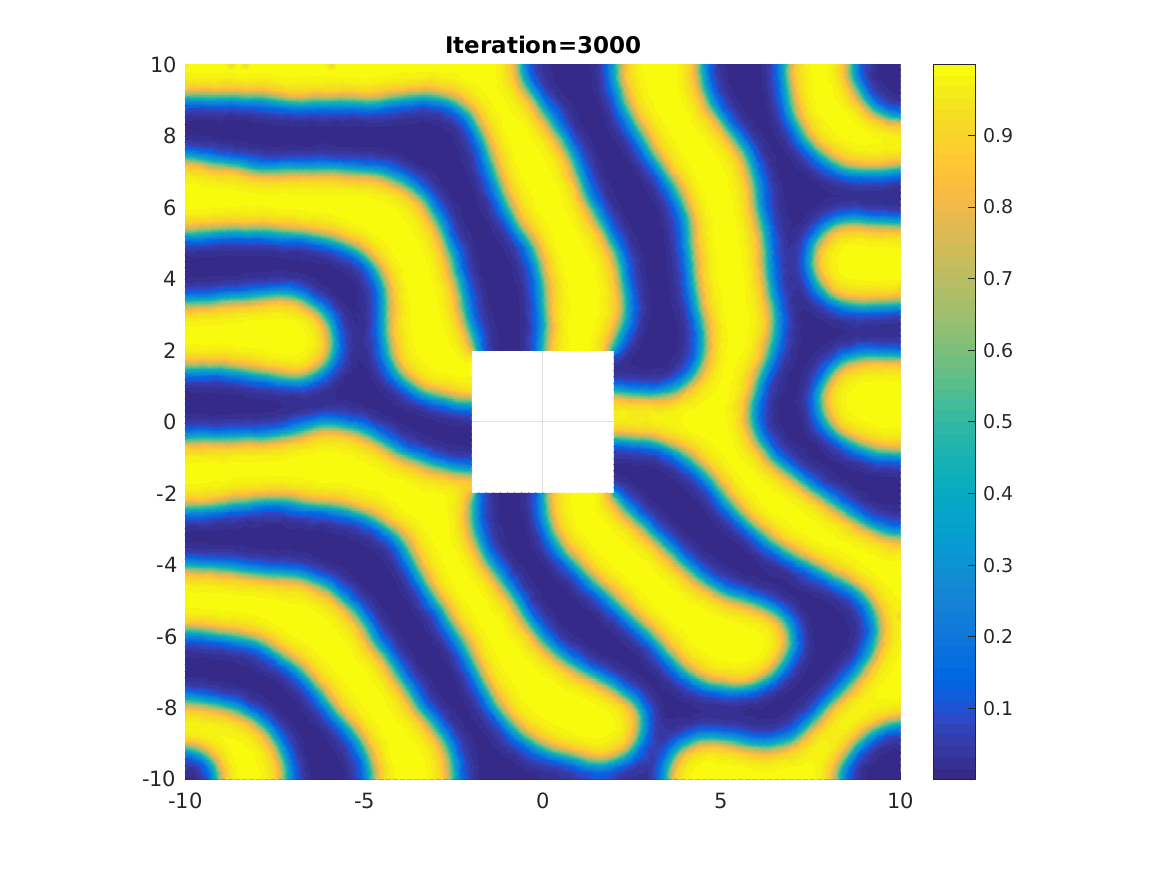
\includegraphics[width=1.2\textwidth]{./figures/01.png}
		\caption{Test1 第3000步迭代图像.}%图片的名称
		\label{fig:liuchengtu1}%标签,用作
	\end{minipage} 
	\hfill
	\begin{minipage}[t]{0.4\linewidth}
		\centering
		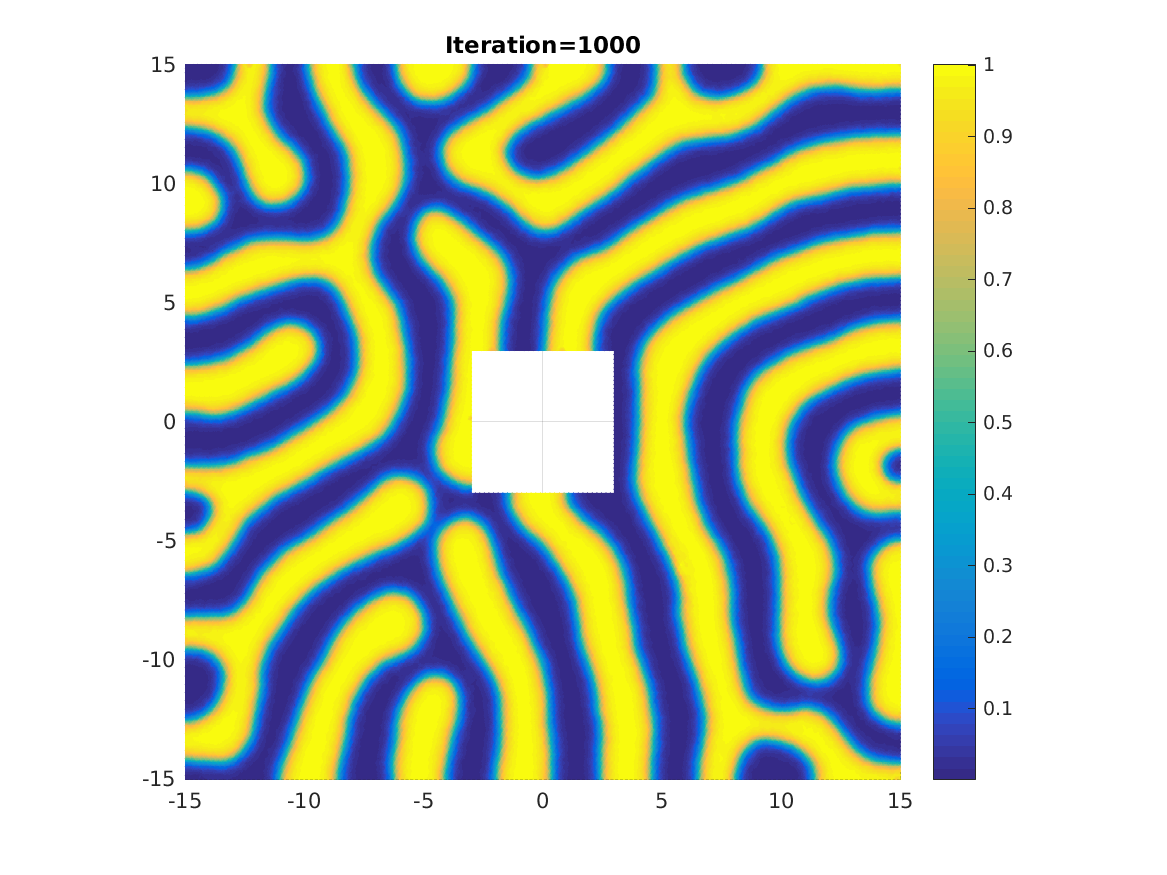
\includegraphics[width=1.2\textwidth]{./figures/02.png}
		\caption{Test2 第1000步迭代图像.}%图片的名称
		\label{fig:liuchengtu2}
	\end{minipage}
    \hfill
    \begin{minipage}[t]{0.4\linewidth}
    	\centering
    	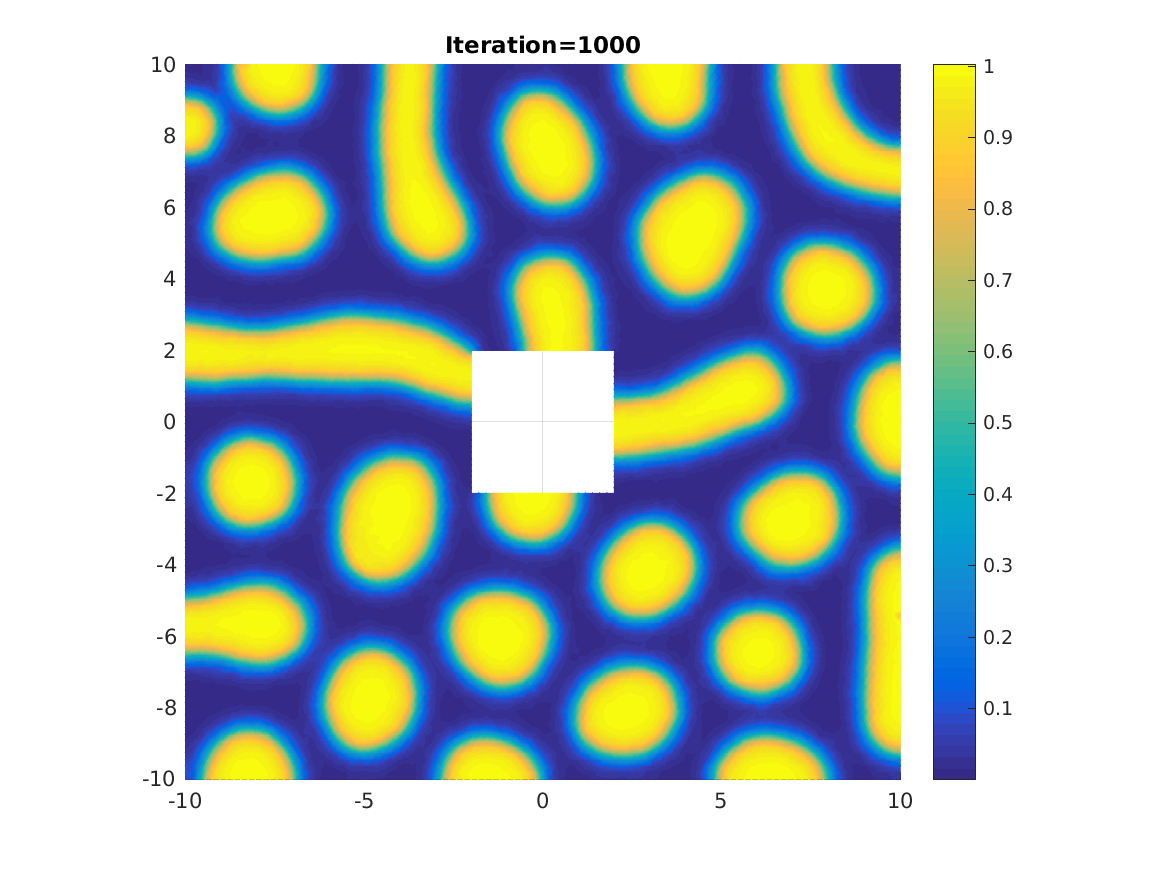
\includegraphics[width=1.2\textwidth]{./figures/03.png}
    	\caption{Test3 第1000步迭代图像.}%图片的名称
    	\label{fig:liuchengtu2}
    \end{minipage}
    \hfill
    \begin{minipage}[t]{0.4\linewidth}
    	\centering
    	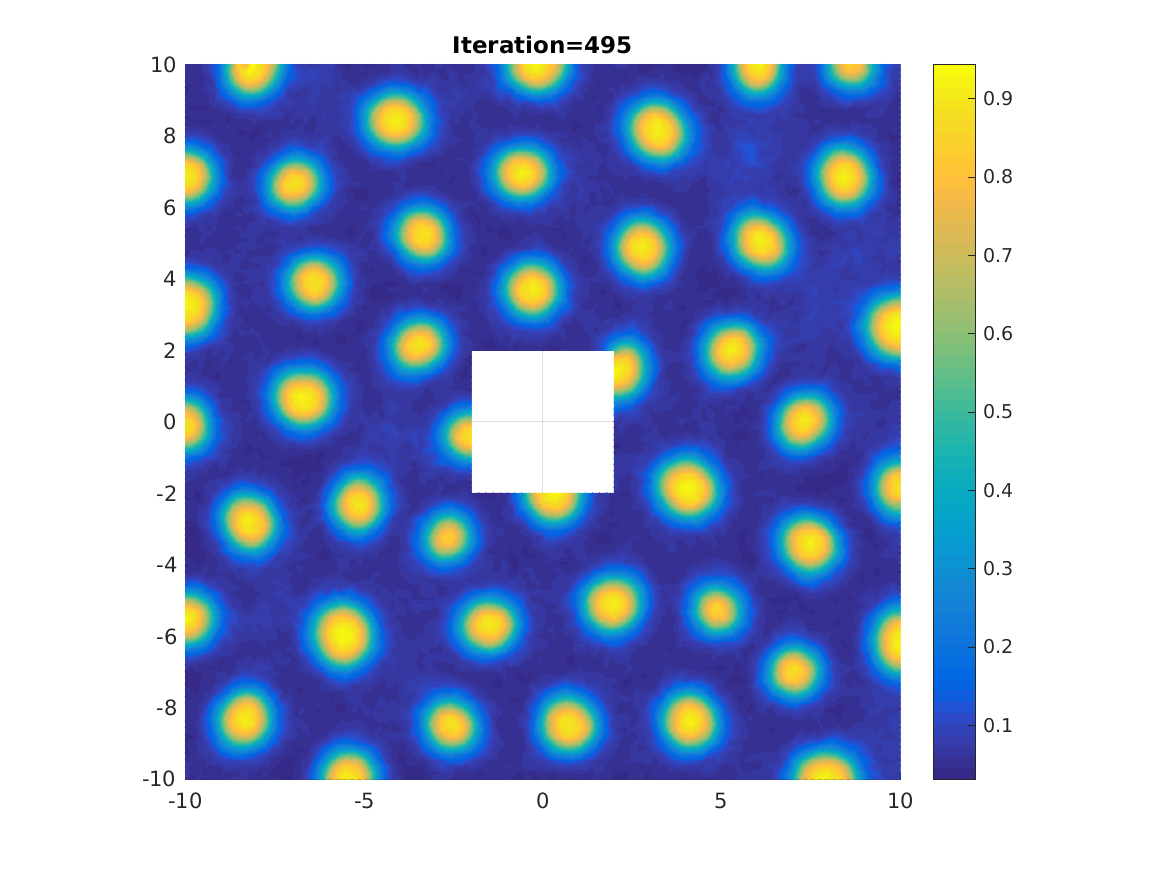
\includegraphics[width=1.2\textwidth]{./figures/04.png}
    	\caption{Test4 第495步迭代图像.}%图片的名称
    	\label{fig:liuchengtu2}
    \end{minipage}
\end{figure}

\newpage
\section{待解决的问题}
1.如何自适应地改变区域,从而重新网格剖分?

如下图所示,首先我们可以手动的改变控制顶点坐标,从而达到目的,但是,当区域复杂或者控制顶点更多时,手动操作则不便于处理,于是我们希望能够自适应地改变区域形状,以达到预期目的。
\begin{figure}[ht]
\centering     %插入的图片居中表示
\begin{minipage}[t]{0.4\linewidth}%并排放两张图片,每张占行的0.4,下同
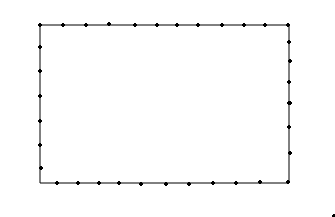
\includegraphics[width=1.2\textwidth]{./figures/figure1.png}
\caption{原始区域.}%图片的名称
\label{fig:liuchengtu1}%标签,用作
\end{minipage} 
\hfill
\begin{minipage}[t]{0.4\linewidth}
\centering
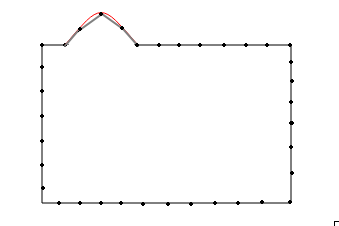
\includegraphics[width=1.2\textwidth]{./figures/figure2.png}
\caption{调整后区域.}%图片的名称
\label{fig:liuchengtu2}
\end{minipage}
\end{figure}


\section{附录}

\subsection{网格剖分函数}

外矩形边长: L

内矩形边长:l  

获取区域函数fd:ddiff(drectangle(p,-L,L,-L,L),drectangle(p,-l,l,-l,l))

网格剖分函数:[p,t]=distmesh2d(fd,fh,h,bbox,pfix]); \%\%fh控制网格类型,h控制网格大小,bbox为最大边界,pfix为控制顶点位置。

有限元网格剖分方法参见:http://persson.berkeley.edu/distmesh/index.html


\subsection{FEniCS使用}

1.Docker安装:

Sudo apt-get update

Sudo apt-get install docker-ce

2.运行FEniCS Docker镜像:

Curl  -s https://get.fenicsproject.org | bash

3.检验:

Sudo docker run hello-world

4.设置镜像:

Sudo docker pull quay.io/fenicsproject/stable:latest

5.启动fenics:

Sudo docker run -ti quay.io/fenicsproject/stable:latest

6.主机与容器文件共享:

Sudo docker run -ti -v\$(pwd):/home/fenics/shared quay.io/fenicsproject/stable:latest
\end{document}
